\annexeToc{\StringGlossaireProprietes}
%cadreIntroductif
\begin{cadre}[A1][A4] 
    Glossaire
    \begin{itemize}
    \item item1
    \item item2
    \item item3
    \item item4
    \end{itemize}
    suite glossaire
\end{cadre}
    

%sections
%001
\titreSectionGlossairePropUn
\ListeProprietes{1} à \ListeProprietes{3}

%002
\titreSectionGlossairePropDeux
\ListeProprietes{4} à \ListeProprietes{7}


\clearpage

\titreSectionGlossairePropUn
\begin{tableau}[pr]{\linewidth}
    \hline %%%%%%%%%%%%%%%%%%%%%%P1 
    \begin{pspicture}(0,0.25)(3.5,2.5)
\pnode(0,0.5){A}
\pnode(2.5,0.5){B}
\pnode(3.5,2){C}
\pnode(1,2){D}
\pspolygon(A)(B)(C)(D)
\psline(A)(C)
\psline(B)(D)
\uput[d](A){$A$}
\uput[d](B){$B$}
\uput[u](C){$C$}
\uput[u](D){$D$}
\end{pspicture}
&
\propriete{} Si un quadrilatère est un parallélogramme alors ses
diagonales se coupent en leur milieu. (C’est aussi vrai pour les
losanges, rectangles et carrés qui sont des parallélogrammes
particuliers.)
&
Ici $ABCD$ est un parallélogramme donc ses diagonales $[AC]$ et
$[BD]$ se coupent en leur milieu.
    
    \\\hline
    \hline %%%%%%%%%%%%%%%%%%%%%%P2 
    \input{\currentpath/inc/section1Propriete002.tex}
    \\\hline
    \hline %%%%%%%%%%%%%%%%%%%%%%P3 
    \input{\currentpath/inc/section1Propriete003.tex}
    \\\hline
\end{tableau}

\titreSectionGlossairePropDeux
\begin{tableau}[pr]{\linewidth}
    \hline %%%%%%%%%%%%%%%%%%%%%%P4 
    Figure
&
\propriete{} Texte
&
Lien figure/propriété

    \\\hline
    \hline %%%%%%%%%%%%%%%%%%%%%%P5 
    \input{\currentpath/inc/section2Propriete005.tex}
    \\\hline
    \hline %%%%%%%%%%%%%%%%%%%%%%P6 
    \input{\currentpath/inc/section2Propriete006.tex}
    \\\hline
    \hline %%%%%%%%%%%%%%%%%%%%%%P7 
    \input{\currentpath/inc/section2Propriete007.tex}
    \\\hline
\end{tableau}

\vfill
\begin{center}
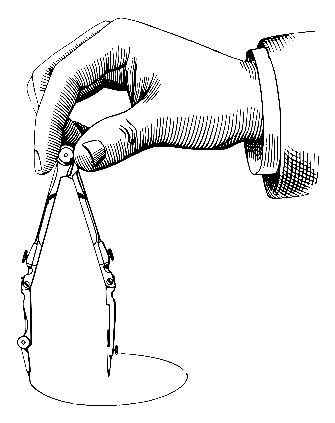
\includegraphics[height=5cm]{\currentpath/images/compas.eps}
% compas.eps: 0x0 pixel, 300dpi, 0.00x0.00 cm, bb=
\end{center}
\vfill
